\documentclass[letterpaper, 10 pt, conference]{ieeeconf}  % Comment this line out if you need a4paper

%\documentclass[a4paper, 10pt, conference]{ieeeconf}      % Use this line for a4 paper

\IEEEoverridecommandlockouts                              % This command is only needed if 
                                                          % you want to use the \thanks command

\overrideIEEEmargins                                      % Needed to meet printer requirements.

%In case you encounter the following error:
%Error 1010 The PDF file may be corrupt (unable to open PDF file) OR
%Error 1000 An error occurred while parsing a contents stream. Unable to analyze the PDF file.
%This is a known problem with pdfLaTeX conversion filter. The file cannot be opened with acrobat reader
%Please use one of the alternatives below to circumvent this error by uncommenting one or the other
%\pdfobjcompresslevel=0
%\pdfminorversion=4

% See the \addtolength command later in the file to balance the column lengths
% on the last page of the document

% The following packages can be found on http:\\www.ctan.org
% \usepackage{graphics} % for pdf, bitmapped graphics files
\usepackage{graphicx}
\usepackage{subcaption}
\usepackage{comment}
\usepackage{epsfig} % for postscript graphics files 
\usepackage{times} % assumes new font selection scheme installed
\usepackage{amsmath} % assumes amsmath package installed
\usepackage{amssymb}  % assumes amsmath package installed
\usepackage{xcolor}
\usepackage{flushend}
\usepackage{booktabs}
\usepackage{cleveref}

\newtheorem{mydef}{\bf Definition}
\newtheorem{mythm}{\bf Theorem}
\newtheorem{myprob}{\bf Problem}
\newtheorem{mylem}{\bf Lemma}
\newtheorem{mycol}{\bf Corollary}
\newtheorem{myprop}{\bf Proposition}
\newtheorem{myexm}{\bf Example}
\newtheorem{remark}{Remark}

\usepackage{algpseudocode}
\usepackage{algorithmicx,algorithm}

\def\XY#1{{\textcolor{red}{ {\bf XY:} #1}}}
% Define a counter for the comments
\newcounter{WSQcomment}
\newcommand{\WSQ}[1]{%
    \stepcounter{WSQcomment} % Increment the counter
    \textcolor{blue}{\#\theWSQcomment\ \textbf{#1}} % Add the number and color the comment
}
\title{\LARGE \bf
% Open-Vocabulary Semantic Safety: Adaptive Conformal Prediction for VLM-based Robot Navigation
Open-World Semantic Safety: Adaptive Conformal Prediction for Zero-Shot Robot Navigation
}
% \title{\LARGE \bf 
% SPARC: Prediction-Based Safe Control for  Coupled Controllable and Uncontrollable Agents with Conformal Predictions}
% \title{\LARGE \bf
% Social Navigation with Conformal Prediction and Robust Guarantee
% }
% \title{\LARGE \bf 
% SPARC: Safe Prediction and Robust Control of Coupled Dynamics}


% \author{Anonymous Authors}
\author{Shuqi Wang, Yue Gao and Xiang Yin}
% <-this % stops a space
% \thanks{This work was supported by the National Natural Science Foundation of China (62173226,62061136004).}% <-this 
% \thanks{Shuqi Wang, Siqi Wang, Shaoyuan Li and Xiang Yin are with Department of Automation and Key Laboratory of System Control and Information Processing, Shanghai Jiao Tong University, Shanghai 200240, China. e-mail: \{wangshuqi, sq\_wang, syli, yinxiang\}@sjtu.edu.cn.}
% stops a space
% \thanks{$^{1}$Albert Author is with Faculty of Electrical Engineering, Mathematics and Computer Science,
%         University of Twente, 7500 AE Enschede, The Netherlands
%         {\tt\small albert.author@papercept.net}}%
% \thanks{$^{2}$Bernard D. Researcheris with the Department of Electrical Engineering, Wright State University,
%         Dayton, OH 45435, USA
%         {\tt\small b.d.researcher@ieee.org}}%



\begin{document}



\maketitle
\thispagestyle{empty}
\pagestyle{empty}


%%%%%%%%%%%%%%%%%%%%%%%%%%%%%%%%%%%%%%%%%%%%%%%%%%%%%%%%%%%%%%%%%%%%%%%%%%%%%%%%
\begin{abstract}

\end{abstract}


\section{INTRODUCTION}

Safe autonomous navigation in semantically rich environments requires maintaining appropriate distances from objects based on their semantic meaning. Recent work has shown that conformal prediction can provide probabilistic safety guarantees for such semantic planning tasks. However, existing approaches build upon closed-set perception models with fixed label spaces and offline calibration, rendering them unable to handle novel semantic concepts that were absent during the calibration phase.
We propose Open-Vocabulary Adaptive Conformal Prediction (OACP), a framework that provides probabilistic semantic safety guarantees for VLM-based robot navigation in open-world environments. By defining nonconformity scores in the VLM's continuous embedding space, our framework ...



\section{Related Works}

\textbf{Zero-Shot Object Navigation.}
Vision-language models (VLMs) have enabled open-vocabulary robotic navigation without task-specific training. VLMaps \cite{huang2023vlmaps} first demonstrated that projecting dense CLIP \cite{radford2021learning} features into a top-down grid map allows robots to interpret natural language goals (e.g., ``I’m thirsty’’ $\to$ navigate to a cup). However, VLMaps requires a complete offline exploration of the environment before constructing the semantic map, precluding real-time deployment. Subsequent work addressed this limitation through online exploration strategies: CoW \cite{gadre2023cows} and ZSON \cite{majumdar2022zson} proposed zero-shot navigation by leveraging CLIP similarities during active exploration; ESC \cite{zhou2023esc} introduced an exploration--exploitation framework that balances frontier exploration with semantic goal pursuit; and VLFM \cite{yokoyama2024vlfm} uses vision-language frontier scoring for efficient goal-directed search. More recently, OneMap \cite{reed2024onemap} introduced a benchmark for zero-shot multi-object navigation, where the robot maintains a semantic map online and leverages information from previous searches to efficiently locate subsequent targets.

Despite this progress, a critical gap remains: \textit{none of these methods account for semantic safety during navigation}. Existing benchmarks evaluate success purely based on whether the robot reaches the target object, ignoring collisions with other objects along the way. In real-world deployment, a robot navigating to a ``bed’’ should not crash into a ``table’’ en route. Our work addresses this gap by introducing semantic safety constraints into the open-vocabulary navigation framework.

\textbf{Conformal Prediction in Control Synthesis.}
Conformal prediction (CP) is a distribution-free framework for constructing prediction sets with finite-sample coverage guarantees \cite{shafer2008tutorial}. Its model-agnostic nature---applicable to any black-box predictor---has made it attractive for safety-critical control, where formal uncertainty quantification is essential.
Recent work has extensively applied CP to control synthesis: Lindemann et al.\ \cite{lindemann2023safe} used CP to construct safe reachable sets for dynamic obstacle avoidance; Yang et al.\ \cite{yang2023safe} extended this to perception-based control under stochastic sensor uncertainty; Dixit et al.\ \cite{dixit2023adaptive} proposed adaptive conformal prediction for motion planning among dynamic agents; and \cite{yu2023,stamouli2024recursively,sun2024conformal} further explored CP-based guarantees in temporal logic planning, shrinking-horizon MPC, and diffusion-based dynamics models, respectively.

Most closely related to our work, Sundarsingh et al.\ \cite{sundarsingh2026safeplanningunknownenvironments} proposed the concept of \textit{semantic safety}---maintaining semantically appropriate distances from objects based on their category---and used conformalized semantic maps to provide probabilistic safety guarantees. However, their approach operates on a \textit{closed} semantic map with a fixed label set and relies on offline calibration. Adding a new object category requires re-calibrating the conformal threshold over the entire label space, making their method unsuitable for open-vocabulary environments where novel objects may be encountered during deployment.

\textbf{Uncertainty Quantification for VLMs.}
Several studies have applied conformal prediction to quantify the uncertainty of vision-language models \cite{kostumov2024uncertaintyawareevaluationvisionlanguagemodels}, revealing that VLM confidence scores are often poorly calibrated---model uncertainty is not aligned with prediction accuracy. However, these analyses are limited to static visual question answering (VQA) benchmarks and do not address how such uncertainty affects downstream decision-making in embodied agents.

Our work bridges these three lines of research. We propose OACP, which provides formal safety guarantees for VLM-based navigation in open-vocabulary environments. By defining nonconformity scores in the VLM’s continuous embedding space rather than over a fixed label set, OACP enables online calibration that remains valid as new semantic concepts are discovered---without requiring map reconstruction or offline re-calibration.


\section{Problem Formulation}

\begin{table*}[h]
\caption{Variable Definitions}
\label{tab:notation}
\centering
\begin{tabular}{l l}
\hline
\textbf{Symbol} & \textbf{Description} \\
\hline
\multicolumn{2}{c}{\textit{Environment and Robot}} \\
$\Omega \subset \mathbb{R}^2$ & Workspace domain \\
$x_t \in \Omega$ & Robot position at time step $t$ \\
$\mathcal{J}$ & Set of indices for the grid map cells \\
$c_j \in \Omega$ & Center position of grid cell $j \in \mathcal{J}$ \\
\hline
\multicolumn{2}{c}{\textit{Open-Vocabulary Semantics and Safety}} \\
$\mathcal{V}_t$ & Open-vocabulary semantic label set at time $t$ \\
$D_{\text{safe}}: \mathcal{V}_t \to \mathbb{R}_{>0}$ & Safety distance function mapped from semantic labels \\
$\phi(\cdot), \psi(\cdot)$ & VLM image and text encoders (e.g., CLIP) \\
$\mathbf{v}_j^{(t)} \in \mathbb{R}^D$ & Aggregated VLM visual embedding for cell $j$ at time $t$ \\
\hline
\multicolumn{2}{c}{\textit{Open-Vocabulary Adaptive Conformal Prediction}} \\
$s(j, l)$ & Nonconformity score: cosine distance in embedding space (Eq.~\ref{eq:nonconf}) \\
$C_t$ & Adaptive nonconformity threshold at time $t$ \\
$\mathcal{C}_j^{(t)} \subseteq \mathcal{V}_t$ & Conformal prediction set: $\{ l \in \mathcal{V}_t \mid s(j, l) \le C_t \}$ \\
$\alpha_t$ & Adaptive risk parameter updated online via ACI \\
$\gamma$ & Step size for the Adaptive Conformal Inference (ACI) update \\
$\mathcal{S}$ & Sliding-window calibration buffer of nonconformity scores \\
$f_{\text{expert}}$ & Delayed expert oracle providing ground-truth labels (Assumption 2) \\
$\tau_j \le \tau_{\max}$ & Bounded delay of expert oracle for cell $j$ \\
\hline
\multicolumn{2}{c}{\textit{Safety-Critical Planning}} \\
$d_{\text{wc}}^{(j)}$ & Worst-case safe distance: $\max_{l \in \mathcal{C}_j^{(t)}} D_{\text{safe}}(l)$ \\
$\mathcal{J}_{\text{obs}}$ & Set of cells identified as obstacles \\
$\mathcal{X}_{\text{safe}}^{(t)}$ & Safe configuration space derived from $d_{\text{wc}}^{(j)}$ \\
\hline
\end{tabular}
\end{table*}

In this section, we formalize the problem of semantic-aware robot navigation in open-world environments. We define the system dynamics, the open-vocabulary semantic environment, and the chance-constrained optimization objective.

\emph{Notations: }We denote $\mathbb{R}, \mathbb{N}$, and $\mathbb{R}^n$ as the set of real numbers, natural numbers, and real vectors, respectively. 
Let $\beta: \mathbb{R} \rightarrow \mathbb{R}$ denote an extended class $\mathcal{K}_{\infty}$ function, i.e., a strictly increasing function with $\beta(0)=0$. 
For a vector $v \in \mathbb{R}^n$, let $|v|$, $\|v\|$, $\|v\|_\infty$ denote its $\ell_1$-norm, Euclidean norm and $\ell_\infty$-norm. 
For a finite set $D$, let $|D|$ denote its cardinality.




\subsection{System Dynamics}
Consider a mobile robot operating in a bounded workspace $\Omega \subset \mathbb{R}^2$. The robot's motion is modeled as a discrete-time nonlinear dynamical system:
\begin{equation}
    x_{k+1} = f(x_k, u_k),
\end{equation}
where $k \in \{0, \dots, H\}$ denotes the time step, $x_k \in \mathcal{X} \subset \mathbb{R}^{n_x}$ represents the robot state (e.g., position and orientation), and $u_k \in \mathcal{U} \subset \mathbb{R}^{n_u}$ denotes the control input constrained by a compact set $\mathcal{U}$.

\subsection{Environment and Semantic Safety}
The environment is discretized into a semantic grid map consisting of $M$ cells, indexed by $\mathcal{J} = \{1, \dots, M\}$. Each cell $j \in \mathcal{J}$ is centered at $c_j \in \Omega$ and is associated with a \textit{ground-truth semantic label} $l_j \in \mathcal{V}$, where $\mathcal{V}$ represents the set of all possible open-vocabulary semantic concepts.

Safety is defined not merely as collision avoidance, but as maintaining semantically appropriate distances from objects. We assume the existence of a ground-truth safety function:
\begin{mydef}[\textbf{Semantic Safety Function}]
    Let $D_{\text{safe}}: \mathcal{V} \to \mathbb{R}_{\ge 0}$ be a function that maps any semantic label $l \in \mathcal{V}$ to a required minimum Euclidean safety margin.
\end{mydef}

Thus, a robot state $x_k$ is considered \textit{semantically safe} with respect to cell $j$ if and only if:
\begin{equation}
    \| x_k - c_j \|_2 \ge D_{\text{safe}}(l_j).
\end{equation}

\subsection{Problem Statement}
The core challenge is that the true label $l_j$ is not directly observable. The robot must infer $l_j$ from noisy Vision-Language Model (VLM) observations. Consequently, deterministic safety cannot be guaranteed.

\textbf{Assumption 1 (Static Environment):} The ground-truth semantic labels $l_j$ of the grid cells do not change during the robot's mission horizon.

We formulate a chance-constrained optimal control problem:

\begin{myprob}
Given a required confidence level $\gamma \in (0, 1)$, our objective is to compute a control sequence that minimizes the path length while ensuring that the probability of violating the semantic safety constraint remains bounded. The optimization problem is formulated as follows:

\begin{subequations}
\label{eq:optimization_problem}
\begin{align}
    % \min_{\mathbf{u}_{0:H-1}} \quad & \sum_{k=0}^{H-1} \| x_{k+1} - x_k \|_2 \\
        \min_{\mathbf{u}_{0:H-1}} \quad & J(\mathbf{x}_{0:H-1},\mathbf{u}_{0:H-1}) \\
    \text{subject to} \quad & x_{k+1} = f(x_k, u_k), \quad \forall k, \\
    & x_0 = x_{\text{init}}, \quad x_H \in \mathcal{X}_{\text{goal}}, \\
    & u_k \in \mathcal{U}, \quad \forall k, \\
    & \mathbb{P}\left( \bigwedge_{j \in \mathcal{J}} \left( \| x_k - c_j \|_2 \ge D_{\text{safe}}(l_j) \right) \right) \ge \gamma, \quad \forall k. \label{eq:chance_constraint}
\end{align}
\end{subequations}

The constraint \eqref{eq:chance_constraint} requires that the joint probability of the robot maintaining the required safety distance from \textit{all} grid cells exceeds $\gamma$ at every time step. In the subsequent sections, we propose a method to convert this intractable chance constraint into a deterministic constraint.

\section{METHODOLOGY}
\label{sec:methodology}

We propose a closed-loop framework that interleaves semantic mapping, uncertainty quantification, and safe planning. The system architecture is illustrated in Fig. \ref{fig:framework}. The core innovation is the Open-Vocabulary Adaptive Conformal Prediction (OACP) module, which calibrates nonconformity scores \textit{in the VLM's continuous embedding space} rather than over a fixed label set. This design choice is the key enabler of open-vocabulary safety: because the calibration operates on embedding-space distances that are independent of the current vocabulary $\mathcal{V}_t$, the conformal threshold remains valid as new semantic concepts are discovered and added online, without requiring map reconstruction or offline recalibration.

\subsection{Embedding Vector-based Semantic Mapping}
\label{subsec:mapping}

We construct a top-down grid map where each cell maintains a high-dimensional semantic feature vector. Let $\phi: \mathbb{R}^{H \times W \times 3} \to \mathbb{R}^D$ and $\psi: \text{Text} \to \mathbb{R}^D$ be the image and text encoders of a pre-trained Vision-Language Model (e.g., CLIP), respectively.

As the robot traverses the environment, we project the ego-centric RGB-D observations into the world coordinate frame. For each grid cell $j \in \mathcal{J}$, we aggregate the visual embeddings of the pixels projected onto it. To handle noise, we employ a running average update. At time $t$, the aggregated feature $\mathbf{v}_j^{(t)}$ for cell $j$ is updated as:
\begin{equation}
    \mathbf{v}_j^{(t)} = \frac{n_j^{(t-1)} \mathbf{v}_j^{(t-1)} + \phi(I_t)_j}{n_j^{(t-1)} + 1},
    \label{eq:vlm_update}
\end{equation}
where $\phi(I_t)_j$ is the embedding of the image patch corresponding to cell $j$ at time $t$, and $n_j$ is the observation count. Crucially, the map stores continuous feature vectors rather than discrete label predictions. This means \textit{the map never needs to be re-rendered when the vocabulary changes}---new labels are simply queried against the existing features via text encoder $\psi$.

\subsection{Open-Vocabulary Adaptive Conformal Prediction (OACP)}
\label{subsec:oacp}

Standard VLM predictions are prone to hallucinations, making raw similarity scores unreliable for safety-critical planning. To satisfy the chance constraint in \eqref{eq:chance_constraint}, we employ conformal prediction to construct valid prediction sets over obstacle labels for each grid cell. Unlike prior work \cite{sundarsingh2026safeplanningunknownenvironments} that calibrates nonconformity scores over a \textit{fixed, closed} label set and requires offline calibration, OACP defines its scores in the VLM's continuous embedding space. This makes the calibration \textit{vocabulary-agnostic}: the conformal threshold $C_t$ governs how far (in cosine distance) a cell's visual embedding must be from any label's text embedding to exclude it from the prediction set. When a new label $l_{\text{new}}$ is added to the vocabulary, $\psi(l_{\text{new}})$ is simply projected into the same embedding space, and the existing threshold $C_t$---already calibrated to control the cosine-distance miscoverage rate---applies to the new label without modification.

\subsubsection{Embedding-Space Non-Conformity Score}
We define the non-conformity score $s(j, l)$ as the cosine distance between the cell's visual embedding and the text embedding of a candidate label $l \in \mathcal{V}_t$:
\begin{equation}
    s(j, l) = 1 - \frac{\mathbf{v}_j^{(t)} \cdot \psi(l)}{\| \mathbf{v}_j^{(t)} \| \| \psi(l) \|}.
    \label{eq:nonconf}
\end{equation}
Lower scores indicate higher semantic similarity. The key distinction from closed-set approaches is that $s(j, l)$ depends only on the geometric relationship between two vectors in the shared embedding space, not on a fixed enumeration of classes. This means the score is well-defined for \textit{any} label $l$ that can be encoded by $\psi$, including labels not present in $\mathcal{V}_t$ at calibration time.

\subsubsection{Conformal Prediction Set and Worst-Case Safety}
For each obstacle cell $j$, the conformal prediction set collects all labels whose nonconformity score falls below the adaptive threshold $C_t$:
\begin{equation}
    \mathcal{C}_j^{(t)} = \left\{ l \in \mathcal{V}_t \;\middle|\; s(j, l) \le C_t \right\}.
    \label{eq:conf_set}
\end{equation}
The robot then plans against the worst-case safety distance within each prediction set:
\begin{equation}
    d_{\text{wc}}^{(j, t)} = \max_{l \in \mathcal{C}_j^{(t)}} D_{\text{safe}}(l).
    \label{eq:wc_dist}
\end{equation}
When $|\mathcal{C}_j^{(t)}| = 1$, the conformal set has collapsed to the single most likely label and the robot uses its exact safety distance. When $|\mathcal{C}_j^{(t)}| > 1$, the robot conservatively plans for the most dangerous plausible label, paying a path-efficiency cost for safety. As calibration improves, $C_t$ tightens, the sets shrink, and the efficiency cost decreases.

\subsubsection{Online Adaptive Conformal Inference (ACI)}
\label{subsubsec:aci}

Online calibration of the threshold $C_t$ requires access to ground-truth labels. We formalize this via a two-tier perception assumption:

\textbf{Assumption 2 (Delayed Expert Oracle):} There exists an expert perception model $f_{\text{expert}}$ that, for any grid cell $j$ observed at time $t$, returns the true semantic label $l_j$ after a bounded delay $\tau_j \le \tau_{\max}$. That is, at time $t + \tau_j$, the label $l_j$ is revealed with certainty. The real-time planning model $f_{\text{real-time}}$ used for online inference may produce noisy or incorrect predictions, but the expert oracle is assumed to be infallible.

\begin{remark}
This two-tier architecture---pairing a lightweight, real-time model for online decision-making with a high-fidelity expert for delayed supervision---reflects a practical paradigm in embodied AI. In deployment, the expert role can be instantiated by heavyweight vision-language models (e.g., Grounding DINO, GPT-4V) whose inference latency precludes real-time use, or by human-in-the-loop verification. The essential requirement is only that ground-truth labels become available after bounded delay; the mechanism is abstracted away. In our experiments, we directly supply ground-truth labels with delay $\tau$ to isolate the conformal calibration module from any specific expert model.
\end{remark}

The nonconformity threshold $C_t$ is calibrated online using Adaptive Conformal Inference (ACI) \cite{gibbs2021adaptive}. When the expert oracle reveals the ground-truth label $l_j$ for a cell $j$ (after delay $\tau_j$), this constitutes a calibration event. The robot maintains a global risk parameter $\alpha_t$ and a sliding-window buffer $\mathcal{S}$ of nonconformity scores from these events.

At each calibration event (cell $j$, true label $l_j$):
\begin{enumerate}
    \item Compute the nonconformity score $s(j, l_j)$ of the true label via Eq.~\eqref{eq:nonconf}. A high score indicates the real-time model's feature was far from the true label's embedding.
    \item Evaluate coverage error under the current threshold:
    \begin{equation}
        \text{err}_t = \mathbb{I}\!\left( s(j, l_j) > C_t \right).
    \end{equation}
    \item Update the risk parameter via the ACI gradient step:
    \begin{equation}
        \alpha_{t+1} = \text{clamp}\!\left( \alpha_t + \gamma \left( \alpha_{\text{target}} - \text{err}_t \right),\; \epsilon,\; 1-\epsilon \right),
        \label{eq:aci_update}
    \end{equation}
    where $\text{clamp}(x, a, b) \triangleq \min(\max(x, a), b)$, $\gamma > 0$ is the step size, $\alpha_{\text{target}} = 1 - \gamma_{\text{safe}}$ is the target miscoverage rate, and $\epsilon > 0$ prevents degeneracy.
    \item Append $s(j, l_j)$ to the calibration buffer $\mathcal{S}$, and update the threshold:
    \begin{equation}
        C_{t+1} = \hat{Q}\!\left(\mathcal{S},\; 1 - \alpha_{t+1}\right),
        \label{eq:tau_update}
    \end{equation}
    where $\hat{Q}(\mathcal{S}, q)$ denotes the $q$-th empirical quantile of the scores in $\mathcal{S}$.
\end{enumerate}
The feedback dynamics are intuitive: when the true label is covered ($\text{err}_t = 0$), $\alpha_t$ increases, $C_t$ tightens, and prediction sets narrow. When coverage fails ($\text{err}_t = 1$), $\alpha_t$ decreases, $C_t$ loosens, and sets broaden. This ensures long-run coverage tracks $1 - \alpha_{\text{target}}$.

\subsection{Open-Vocabulary Safety Dictionary}
\label{subsec:open_vocab}

The embedding-space formulation of OACP enables a capability that is fundamentally impossible in closed-set conformal prediction: the safety dictionary $(\mathcal{V}_t, D_{\text{safe}})$ can be expanded online without invalidating the calibration.

\subsubsection{Why Embedding-Space Calibration Enables Open Vocabulary}

In prior closed-set approaches \cite{sundarsingh2026safeplanningunknownenvironments}, the nonconformity score is defined as the softmax rank or class probability of the true label within a fixed label space $\mathcal{V} = \{l_1, \dots, l_K\}$. The conformal threshold is calibrated to control miscoverage over this specific $K$-class classification problem. Adding a new label $l_{K+1}$ fundamentally changes the classification task---the softmax distribution shifts, the calibration scores become stale, and the coverage guarantee is voided.

In OACP, the nonconformity score $s(j, l)$ in Eq.~\eqref{eq:nonconf} measures a pairwise cosine distance in embedding space. This score does not depend on what other labels exist in $\mathcal{V}_t$: adding $l_{K+1}$ does not change $s(j, l_k)$ for any existing $k \le K$. The threshold $C_t$ has been calibrated to control the rate at which the true label's embedding falls further than $C_t$ from the visual feature---a geometric property that is invariant to the vocabulary size. Therefore, $C_t$ remains a valid coverage controller even after vocabulary expansion. This contrast is illustrated in Fig.~\ref{fig:oacp_insight}.

\begin{figure*}[t]
    \centering
    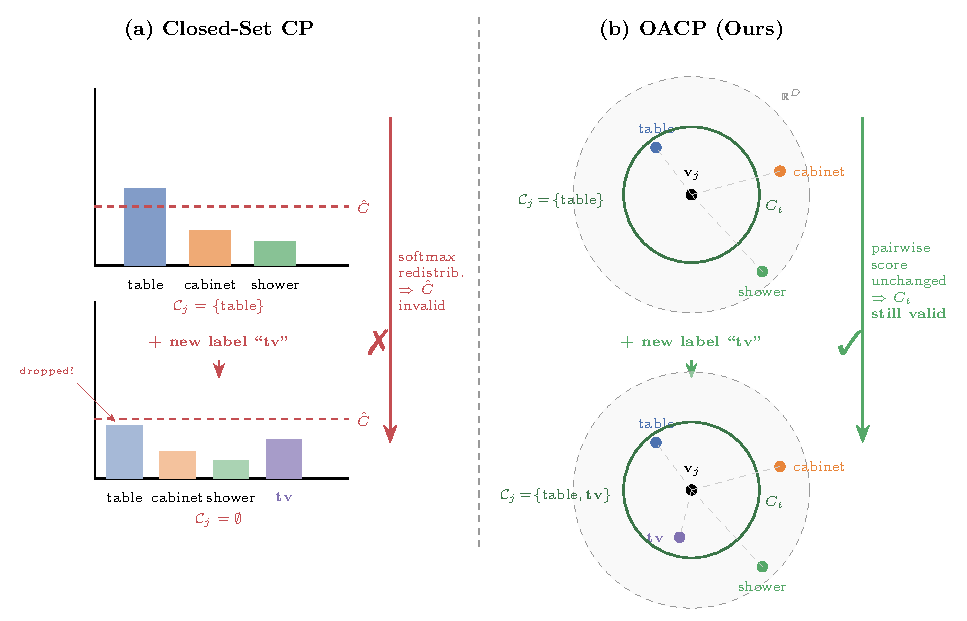
\includegraphics[width=\textwidth]{fig/fig_motivation.pdf}
    \caption{Closed-set CP vs.\ OACP under vocabulary expansion. \textbf{(a)}~In closed-set CP, adding a new label $l_{K+1}$ redistributes the softmax probabilities, causing the previously covered true label to drop below the calibrated threshold $\hat{C}$---the prediction set becomes empty and coverage is lost. \textbf{(b)}~In OACP, the nonconformity score $s(j,l)$ (Eq.~\ref{eq:nonconf}) is a pairwise cosine distance in embedding space. Adding $l_{K+1}$ introduces a new point without affecting existing distances, so the threshold $C_t$ remains valid and the prediction set naturally expands to include the new label.}
    \label{fig:oacp_insight}
\end{figure*}

\subsubsection{Monotonic Dictionary Expansion}

OACP can operate with an initially empty obstacle vocabulary $\mathcal{V}_0 = \emptyset$. As the robot navigates and the expert oracle (Assumption~2) reveals ground-truth labels, new obstacle concepts are discovered and registered. When the expert identifies a label $l_{\text{new}} \notin \mathcal{V}_t$ for the first time:
\begin{enumerate}
    \item \textbf{Label Registration:} The text embedding $\psi(l_{\text{new}})$ is computed and appended to the obstacle embedding matrix.
    \item \textbf{Safety Radius Assignment:} The safety distance $D_{\text{safe}}(l_{\text{new}})$ is provided by the expert or an external safety assessor.
    \item \textbf{Dictionary Update:} $\mathcal{V}_{t+1} \leftarrow \mathcal{V}_t \cup \{l_{\text{new}}\}$.
\end{enumerate}
This expansion is \textit{strictly additive}: once a semantic concept and its safety margin are registered, they are immutable and cannot be removed. This monotonicity ensures that the safe configuration space $\mathcal{X}_{\text{safe}}^{(t)}$ can only become more conservative (or stay the same) when new hazards are discovered, preventing safety regression from forgetting.

Immediately after expansion, the new label participates in conformal set construction \eqref{eq:conf_set} for all cells: $\psi(l_{\text{new}})$ is compared against every stored visual feature $\mathbf{v}_j^{(t)}$ using the existing threshold $C_t$. No map re-rendering, feature re-extraction, or recalibration is required.

The complete OACP procedure is summarized in Algorithm~\ref{alg:oacp}.

\begin{algorithm}[t]
\caption{Open-Vocabulary Adaptive Conformal Prediction (OACP)}
\label{alg:oacp}
\hspace*{0.02in} {\bf Input:}
Feature map $\{\mathbf{v}_j^{(t)}\}$; Robot state $x_t$; Obstacle dictionary $(\mathcal{V}_t, D_{\text{safe}})$; Threshold $C_t$; Risk $\alpha_t$; Buffer $\mathcal{S}$; Step size $\gamma$; Target $\alpha_{\text{target}}$; Near-field radius $\delta_{\text{obs}}$\\
\hspace*{0.02in} {\bf Output:}
Updated $(\mathcal{V}_{t+1}, C_{t+1}, \alpha_{t+1})$; Worst-case safety map
\begin{algorithmic}[1]
\State \textit{// Phase 1: Expert oracle feedback \& dictionary expansion}
\For{each cell $j$ where expert reveals GT label $l_j$ (Assumption 2)}
    \If{$l_j \notin \mathcal{V}_t$} \Comment{Open-vocabulary discovery}
        \State Compute $\psi(l_j)$; assign $D_{\text{safe}}(l_j)$ from expert
        \State $\mathcal{V}_t \gets \mathcal{V}_t \cup \{l_j\}$ \Comment{Monotonic expansion}
    \EndIf
    \State \textit{// ACI calibration (Eq.~\ref{eq:nonconf})}
    \State $s \gets s(j, l_j)$ \Comment{Nonconformity score}
    \State $\text{err} \gets \mathbb{I}(s > C_t)$
    \State $\alpha_t \gets \text{clamp}(\alpha_t + \gamma(\alpha_{\text{target}} - \text{err}),\; \epsilon,\; 1-\epsilon)$
    \State $\mathcal{S} \gets \mathcal{S} \cup \{s\}$;\; $C_t \gets \hat{Q}(\mathcal{S},\; 1 - \alpha_t)$
\EndFor

\vspace{0.05in}
\State \textit{// Phase 2: Conformal prediction sets \& worst-case safety}
\For{each obstacle cell $j$}
    \State $\mathcal{C}_j \gets \{l \in \mathcal{V}_t \mid s(j,l) \le C_t\}$ \Comment{Prediction set}
    \State $d_{\text{wc}}^{(j)} \gets \max_{l \in \mathcal{C}_j} D_{\text{safe}}(l)$ \Comment{Worst-case radius}
    \State Dilate cell $j$ by $d_{\text{wc}}^{(j)}$ on obstacle map
\EndFor
\end{algorithmic}
\end{algorithm}

\subsection{Safety-Critical Planning}
\label{subsec:planning}

The output of the OACP module is a worst-case obstacle map where each obstacle cell $j$ is dilated by its safety radius $d_{\text{wc}}^{(j, t)}$.

The safe configuration space at time $t$ is defined as:
\begin{equation}
    \mathcal{X}_{\text{safe}}^{(t)} = \left\{ x \in \Omega \;\middle|\; \forall j \in \mathcal{J}_{\text{obs}},\; \| x - c_j \| \ge d_{\text{wc}}^{(j, t)} \right\},
\end{equation}
where $\mathcal{J}_{\text{obs}} \subseteq \mathcal{J}$ denotes the set of cells identified as obstacles.

We solve the trajectory optimization problem defined in \eqref{eq:optimization_problem} using a graph-based planner (A* with Fast Marching Method) on the discretized grid. The dilated obstacle map directly encodes $\mathcal{X}_{\text{safe}}^{(t)}$, so the planner naturally generates trajectories satisfying the probabilistic safety constraints. As the ACI module accumulates calibration data, the conformal sets $\mathcal{C}_j^{(t)}$ narrow and the navigable space expands, yielding more efficient paths over time.

\end{myprob}\medskip


% \subsection{Long-Run Coverage Guarantee}
% Seeing ACI.

% \subsection{Probabilistic Safety Satisfaction}
% Obviously.
\section{THEORETICAL ANALYSIS}
\label{sec:analysis}

In this section, we provide theoretical guarantees for the proposed framework. We first establish long-run coverage for the standard (no-delay) ACI update following Gibbs and Cand\`es \cite{gibbs2021adaptive}, then extend the analysis to the delayed-feedback setting arising from Assumption~2, and finally show that coverage translates into probabilistic safety.

Throughout this section, we write $\alpha \triangleq \alpha_{\text{target}}$ for brevity. Recall the ACI update:
\begin{equation}
    \alpha_{t+1} = \alpha_t + \gamma(\alpha - \text{err}_t).
    \label{eq:aci_recall}
\end{equation}

\subsection{Coverage Guarantee without Delay}

We first recall the standard ACI guarantee.

\begin{mylem}[\textbf{Boundedness of $\alpha_t$} {\cite[Lemma~4.1]{gibbs2021adaptive}}]
\label{lem:bound_nodelay}
With probability one, $\alpha_t \in [-\gamma, 1+\gamma]$ for all $t \in \mathbb{N}$.
\end{mylem}

\begin{proof}
Assume by contradiction that with positive probability $\inf_t \alpha_t < -\gamma$ (the case $\sup_t \alpha_t > 1+\gamma$ is symmetric). Since $\sup_t |\alpha_{t+1} - \alpha_t| = \sup_t \gamma|\alpha - \text{err}_t| \le \gamma$, with positive probability we can find $t$ such that $\alpha_t < 0$ and $\alpha_{t+1} < \alpha_t$. However,
\begin{equation}
    \alpha_t < 0 \;\Longrightarrow\; \hat{Q}_t(1-\alpha_t) = \infty \;\Longrightarrow\; \text{err}_t = 0 \;\Longrightarrow\; \alpha_{t+1} = \alpha_t + \gamma\alpha \ge \alpha_t,
\end{equation}
contradicting $\alpha_{t+1} < \alpha_t$. Hence $\mathbb{P}(\exists t: \alpha_{t+1} < \alpha_t < 0) = 0$.
\end{proof}

\begin{myprop}[\textbf{Long-Run Coverage} {\cite[Prop.~4.1]{gibbs2021adaptive}}]
\label{prop:coverage_nodelay}
With probability one, for all $T \in \mathbb{N}$,
\begin{equation}
    \left| \frac{1}{T} \sum_{t=1}^T \text{err}_t - \alpha \right| \le \frac{\max\{\alpha_1,\, 1-\alpha_1\} + \gamma}{T\gamma}.
    \label{eq:coverage_nodelay}
\end{equation}
In particular, $\lim_{T \to \infty} \frac{1}{T}\sum_{t=1}^T \text{err}_t = \alpha$ almost surely.
\end{myprop}

\begin{proof}
Expanding the recursion \eqref{eq:aci_recall} and applying Lemma~\ref{lem:bound_nodelay}:
\begin{equation}
    [-\gamma, 1+\gamma] \ni \alpha_{T+1} = \alpha_1 + \sum_{t=1}^T \gamma(\alpha - \text{err}_t).
\end{equation}
Rearranging gives the result.
\end{proof}

\subsection{Coverage Guarantee under Feedback Delay}
\label{subsec:convergence_delay}

As formalized in Assumption~2, the expert oracle reveals the ground-truth label for cell $j$ after a bounded delay $\tau_j \le k$, where $k \triangleq \tau_{\max}$. Therefore, at time step $t$ the ACI update uses the coverage error from step $t - k + 1$:
\begin{equation}
    \alpha_{t+1} = \alpha_t + \gamma(\alpha - \text{err}_{t-k+1}).
    \label{eq:aci_delay}
\end{equation}
Below we show that the long-run coverage guarantee is preserved with an enlarged but vanishing transient term proportional to $k$.

\begin{mylem}[\textbf{Boundedness of $\alpha_t$ under Delay}]
\label{lem:bound_delay}
Under the delayed update \eqref{eq:aci_delay} with initialization $\alpha_0 \in [0,1]$, with probability one,
\begin{equation}
    \alpha_t \in \bigl[-k\gamma(1-\alpha),\; 1 + k\gamma\alpha\bigr] \subseteq [-k\gamma,\; 1+k\gamma], \quad \forall t \in \mathbb{N}.
\end{equation}
\end{mylem}

\begin{proof}
\textbf{Lower bound.}
We show $\alpha_t \ge -k\gamma(1-\alpha)$ for all $t$. For any $t$ with $\alpha_t < 0$, let $t_0 \le t$ be the last time at which $\alpha_{t_0} \ge 0$ (such $t_0$ exists since $\alpha_0 \in [0,1]$). By definition, $\alpha_s < 0$ for all $s \in \{t_0+1, \dots, t\}$. We consider two cases.

\emph{Case 1:} $t - t_0 \le k$. Each update satisfies $\alpha_{s+1} - \alpha_s = \gamma(\alpha - \text{err}_{s-k+1}) \ge -\gamma(1-\alpha)$, so
\begin{equation}
    \alpha_t \ge \alpha_{t_0} - (t-t_0)\,\gamma(1-\alpha) \ge 0 - k\gamma(1-\alpha).
\end{equation}

\emph{Case 2:} $t - t_0 > k$. Split the telescoping sum $\alpha_t - \alpha_{t_0} = \sum_{s=t_0}^{t-1} \gamma(\alpha - \text{err}_{s-k+1})$ into two parts. For $s \in \{t_0, \dots, t_0+k-1\}$, each term is bounded below by $-\gamma(1-\alpha)$, contributing at least $-k\gamma(1-\alpha)$. For $s \ge t_0+k$, the index $s - k + 1 \ge t_0 + 1$, so $\alpha_{s-k+1} < 0$ by the definition of $t_0$. Since $\alpha_{s-k+1} < 0$ implies $\hat{Q}(1-\alpha_{s-k+1}) = \infty$ and hence $\text{err}_{s-k+1} = 0$, each of these terms equals $\gamma\alpha > 0$. Therefore,
\begin{equation}
    \alpha_t \ge \alpha_{t_0} - k\gamma(1-\alpha) + (t - t_0 - k)\gamma\alpha \ge 0 - k\gamma(1-\alpha) + 0.
\end{equation}

In both cases, $\alpha_t \ge -k\gamma(1-\alpha)$.

\textbf{Upper bound.}
The argument is symmetric. For any $t$ with $\alpha_t > 1$, let $t_0 \le t$ be the last time with $\alpha_{t_0} \le 1$. For $s \ge t_0 + k$, the index $s-k+1 \ge t_0+1$ gives $\alpha_{s-k+1} > 1$, so $\hat{Q}(1-\alpha_{s-k+1}) = -\infty$, the prediction set is empty, and $\text{err}_{s-k+1} = 1$. Each such term equals $\gamma(\alpha - 1) = -\gamma(1-\alpha) < 0$, which opposes further increase. The worst-case overshoot occurs in the first $\min(t-t_0, k)$ steps, each contributing at most $\gamma\alpha$, giving $\alpha_t \le 1 + k\gamma\alpha$.
\end{proof}

\begin{myprop}[\textbf{Long-Run Coverage under Delay}]
\label{prop:coverage_delay}
Under the delayed update \eqref{eq:aci_delay}, with probability one, for all $T \in \mathbb{N}$,
\begin{equation}
    \left| \frac{1}{T} \sum_{t=1}^T \text{err}_t - \alpha \right| \le \frac{\max\{\alpha_k,\, 1-\alpha_k\} + k\gamma}{T\gamma}.
    \label{eq:coverage_delay}
\end{equation}
In particular, $\lim_{T \to \infty} \frac{1}{T}\sum_{t=1}^T \text{err}_t = \alpha$ almost surely.
\end{myprop}

\begin{proof}
Summing the delayed update \eqref{eq:aci_delay} from $t = k$ to $T+k-1$:
\begin{equation}
    \sum_{t=k}^{T+k-1} (\alpha_{t+1} - \alpha_t) = \sum_{t=k}^{T+k-1} \gamma(\alpha - \text{err}_{t-k+1}).
\end{equation}
The left-hand side telescopes to $\alpha_{T+k} - \alpha_k$. Substituting $j = t - k + 1$ on the right:
\begin{equation}
    \alpha_{T+k} - \alpha_k = \gamma \sum_{j=1}^{T} (\alpha - \text{err}_j).
\end{equation}
Dividing by $T\gamma$ and rearranging:
\begin{equation}
    \frac{1}{T}\sum_{j=1}^{T} \text{err}_j - \alpha = \frac{\alpha_k - \alpha_{T+k}}{T\gamma}.
\end{equation}
Taking absolute values and applying Lemma~\ref{lem:bound_delay}:
\begin{align}
    |\alpha_k - \alpha_{T+k}| &\le \max\bigl\{(1-\alpha_k) + k\gamma\alpha,\; \alpha_k + k\gamma(1-\alpha)\bigr\} \nonumber \\
    &\le \max\{1-\alpha_k,\; \alpha_k\} + k\gamma.
\end{align}
This yields the stated bound.
\end{proof}

\begin{remark}[\textbf{Effect of Delay}]
Comparing \eqref{eq:coverage_nodelay} with \eqref{eq:coverage_delay}, the delay $k$ inflates the transient numerator from $\gamma$ to $k\gamma$. However, the bound is $O(1/T)$ regardless of $k$, so asymptotic coverage is unaffected:
\begin{equation}
    \lim_{T \to \infty} \frac{1}{T}\sum_{t=1}^T \text{err}_t = \alpha_{\text{target}}, \quad \text{a.s.}
\end{equation}
In practice, larger $k$ means slower convergence during the transient phase; the effective convergence time scales as $O(k/\gamma)$ rather than $O(1/\gamma)$.
\end{remark}

\subsection{Probabilistic Safety Guarantee}
We now link the semantic coverage to the physical safety constraints defined in Eq. \eqref{eq:chance_constraint}.

\begin{mythm}[\textbf{Semantic Safety}]
\label{thm:safety}
Consider a grid cell $j$ with true label $l_j$. Let $\mathcal{C}_j^{(t)}$ be a valid prediction set such that $\mathbb{P}(l_j \in \mathcal{C}_j^{(t)}) \ge 1 - \alpha_{\text{target}}$. If the robot state $x_t$ satisfies the worst-case safety constraint:
\begin{equation}
    \| x_t - c_j \| \ge d_{\text{wc}}^{(j,t)} = \max_{l \in \mathcal{C}_j^{(t)}} D_{\text{safe}}(l),
\end{equation}
then the probability of violating the true semantic safety distance is bounded by $\alpha_{\text{target}}$.
\end{mythm}

\begin{proof}
Let $E = \{ l_j \in \mathcal{C}_j^{(t)} \}$. By assumption, $\mathbb{P}(E) \ge 1 - \alpha_{\text{target}}$.
Conditioned on $E$:
\begin{equation}
    D_{\text{safe}}(l_j) \le \max_{l \in \mathcal{C}_j^{(t)}} D_{\text{safe}}(l) = d_{\text{wc}}^{(j,t)}.
\end{equation}
Since the planner ensures $\| x_t - c_j \| \ge d_{\text{wc}}^{(j,t)}$, event $E$ implies $\| x_t - c_j \| \ge D_{\text{safe}}(l_j)$.
Let $V$ be the violation event $\| x_t - c_j \| < D_{\text{safe}}(l_j)$. Then $V \subseteq \neg E$, and $\mathbb{P}(V) \le \mathbb{P}(\neg E) \le \alpha_{\text{target}}$.
\end{proof}

\begin{remark}
Theorem \ref{thm:safety} provides a marginal guarantee for a single cell. For the full trajectory, satisfying the joint chance constraint \eqref{eq:chance_constraint} strictly requires applying a union bound (e.g., setting $\alpha_{\text{target}} \approx \gamma / M$). In practice, the marginal adaptation is sufficient for robust navigation, as demonstrated in our experiments.
\end{remark}






\section{EXPERIMENTS}
\label{sec:experiments}

We evaluate the proposed OACP framework on the Matterport3D (MP3D) dataset \cite{chang2017matterport3d} using the Habitat simulator \cite{savva2019habitat}. All experiments use a common zero-shot multi-object navigation pipeline with GCLIP dense features for the semantic map and ConvNeXt-CLIP for goal navigation.

\subsection{Setup}

\textbf{Dataset and metrics.}
We use $N=128$ multi-object navigation episodes from the MP3D validation set. Each episode specifies a sequence of target objects; the robot must navigate to each in turn. We report:
\begin{itemize}
    \item \textit{Success Rate (SR)}: fraction of episodes where all targets are reached.
    \item \textit{Semantic Collision Rate (SCR)}: fraction of episodes terminated due to violating a semantic safety constraint (entering the safety zone of an obstacle object).
    \item \textit{STUCK Rate}: fraction of episodes where the planner fails to find a valid path (over-conservative obstacle maps block all routes).
\end{itemize}

SR measures task performance; SCR measures safety violations; STUCK rate measures over-conservatism. An ideal system maximizes SR while minimizing both SCR and STUCK.

\textbf{Semantic safety specification.}
We define 5 obstacle categories with heterogeneous safety radii (in grid cells at $0.1$\,m/cell): \texttt{shower}~(3), \texttt{cabinet}~(4), \texttt{chest of drawers}~(4), \texttt{table}~(5), \texttt{tv}~(2). A semantic collision occurs when the robot enters the dilated safety zone of any obstacle. The evaluation uses ground-truth object locations from the simulator as the oracle.

\textbf{Conditions.}
The robot has no prior knowledge of the environment. All obstacle categories are unknown at deployment time and must be discovered online. We compare three conditions on the same 128 episodes:
\begin{enumerate}
    \item[\textbf{A.}] \textbf{Baseline (OneMap):} Standard OneMap \cite{reed2024onemap} navigation with YOLO-based obstacle detection. No VLM-based semantic obstacle map.
    \item[\textbf{B.}] \textbf{GCLIP Argmax:} GCLIP dense features for obstacle detection. The obstacle dictionary is initialized empty and expanded online via the expert oracle (Assumption~2). A fixed confidence threshold ($\tau = 0.30$) gates detection; no conformal prediction.
    \item[\textbf{C.}] \textbf{OACP (Ours):} Same empty-dictionary initialization as B. Full OACP pipeline with ACI-calibrated threshold ($\gamma_{\text{safe}} = 0.9$, $\gamma = 0.05$), worst-case radius from conformal prediction sets.
\end{enumerate}
All three use the same VLM backbone (ConvNeXt-CLIP for navigation, GCLIP for obstacle detection) and identical planner parameters.

\subsection{Main Results}

\begin{table}[t]
\caption{Navigation results on 128 MP3D episodes (common episode set). SR = Success Rate, SCR = Semantic Collision Rate, STUCK = planner deadlock rate. Best safety in \textbf{bold}.}
\label{tab:main_results}
\centering
\begin{tabular}{lccc}
\toprule
\textbf{Method} & \textbf{SR} $\uparrow$ & \textbf{SCR} $\downarrow$ & \textbf{STUCK} $\downarrow$ \\
\midrule
A. Baseline (OneMap) & 26.6\% & 26.6\% & 20.3\% \\
B. GCLIP Argmax      & 18.0\% & 14.8\% & 25.8\% \\
C. OACP (Ours)       & 10.2\% & \textbf{7.0\%}  & 40.6\% \\
\bottomrule
\end{tabular}
\end{table}

Table~\ref{tab:main_results} presents the main results. The key findings are:

\textbf{OACP achieves the lowest collision rate.}
OACP reduces the semantic collision rate from $26.6\%$ (Baseline) to $\mathbf{7.0\%}$, a $\mathbf{73.7\%}$ relative reduction. Compared to GCLIP Argmax ($14.8\%$), OACP achieves a further $52.7\%$ reduction. This confirms that the worst-case conformal prediction sets effectively inflate safety margins where label uncertainty is high.

\textbf{Safety-efficiency tradeoff.}
The improved safety comes at the cost of increased STUCK rate ($40.6\%$ vs. $20.3\%$ for Baseline), reflecting the conservative nature of worst-case radius assignment. When $|\mathcal{C}_j| > 1$, the robot plans against the largest safety radius in the prediction set, which can over-block narrow passages. As predicted by the theory, this conservatism decreases as calibration improves and the conformal sets shrink.

\textbf{Argmax provides a strong detection backbone.}
The GCLIP Argmax condition already halves the collision rate compared to Baseline ($14.8\%$ vs. $26.6\%$), confirming that the VLM embedding space provides a useful detection signal even without conformal calibration. OACP builds on this backbone by adding uncertainty-aware safety margins.

% TODO: Open-vocabulary ablation — pending full-dataset experiment results



\section{Conclusion}


\bibliographystyle{IEEEtran}
\bibliography{ref}

% \newpage
% \section*{Appendix}
% % \subsection{Simulation Parameters}

  


\end{document}
